\documentclass{standalone}
\usepackage{tikz}
\usetikzlibrary{calc,intersections}
\usepackage{animate}
\begin{document}
%==================
%\pagecolor{black}
%\begin{animateinline}[controls,autoplay,palindrome,loop]{16}
%\multiframe{90}{i=90+1}{
\foreach \i in {0}{
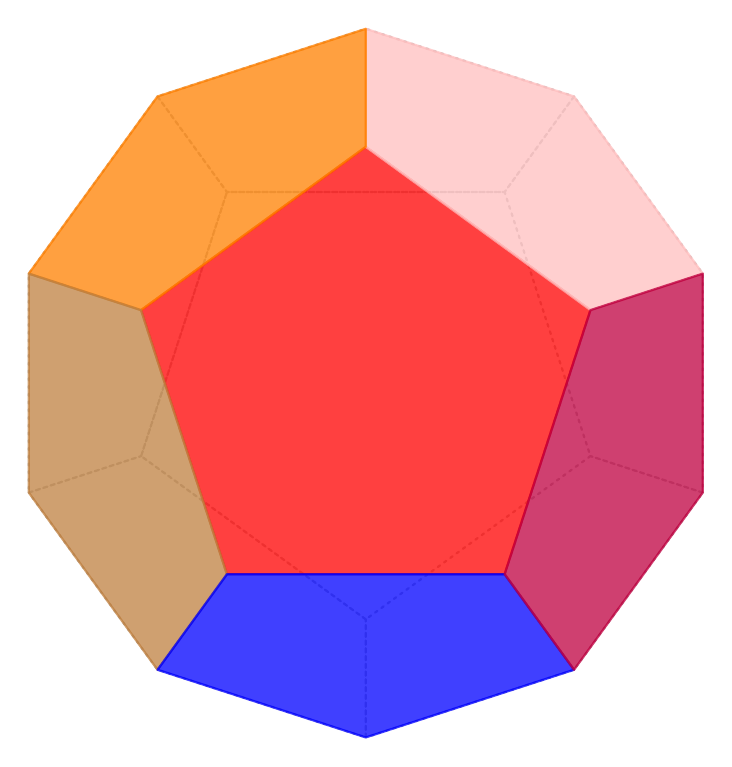
\begin{tikzpicture}[join=round,cap=round,thick]
\def\r{3}
\def\gA{18}
\path
(\gA:\r) coordinate (A_1)
(\gA+72:\r) coordinate (A_2)
(\gA+144:\r) coordinate (A_3)
(\gA+216:\r) coordinate (A_4)
(\gA+288:\r) coordinate (A_5)
(\gA+36:\r) coordinate (B_1)
(\gA+108:\r) coordinate (B_2)
(\gA+180:\r) coordinate (B_3)
(\gA+252:\r) coordinate (B_4)
(\gA+324:\r) coordinate (B_5)
\foreach \i in {1,...,10}{(\gA+\i *36-36:1.5*\r) coordinate (C_\i)}
;
\draw[dotted,opacity=.25] 
(B_1)--(B_2)--(B_3)--(B_4)--(B_5)--cycle
(B_1)--(C_2)--(C_3)--(C_4)--(B_2)--cycle
(B_2)--(C_4)--(C_5)--(C_6)--(B_3)--cycle
(B_3)--(C_6)--(C_7)--(C_8)--(B_4)--cycle
(B_4)--(C_8)--(C_9)--(C_10)--(B_5)--cycle
(B_5)--(C_10)--(C_1)--(C_2)--(B_1)--cycle
;

%\draw[yellow,fill=yellow,opacity=.25] (B_1)--(B_2)--(B_3)--(B_4)--(B_5)--cycle;
%\draw[blue,fill=blue,opacity=.25] (B_1)--(C_2)--(C_3)--(C_4)--(B_2)--cycle;
%\draw[purple,fill=purple,opacity=.25] (B_2)--(C_4)--(C_5)--(C_6)--(B_3)--cycle;
%\draw[pink,fill=pink,opacity=.25] (B_3)--(C_6)--(C_7)--(C_8)--(B_4)--cycle;
%\draw[orange,fill=orange,opacity=.25] (B_4)--(C_8)--(C_9)--(C_10)--(B_5)--cycle;
%\draw[brown,fill=brown,opacity=.25] (B_5)--(C_10)--(C_1)--(C_2)--(B_1)--cycle;
\draw[red,fill=red,opacity=.75] (A_1)--(A_2)--(A_3)--(A_4)--(A_5)--cycle;
\draw[pink,fill=pink,opacity=.75] (A_1)--(C_1)--(C_2)--(C_3)--(A_2)--cycle;
\draw[orange,fill=orange,opacity=.75] (A_2)--(C_3)--(C_4)--(C_5)--(A_3)--cycle;
\draw[brown,fill=brown,opacity=.75] (A_3)--(C_5)--(C_6)--(C_7)--(A_4)--cycle;
\draw[blue,fill=blue,opacity=.75] (A_4)--(C_7)--(C_8)--(C_9)--(A_5)--cycle;
\draw[purple,fill=purple,opacity=.75] (A_5)--(C_9)--(C_10)--(C_1)--(A_1)--cycle;
\end{tikzpicture}

}
%\end{animateinline}

\end{document}
